\intro{
Gli esercizi svolti relativi a questo capitolo sono disponibili su GitHub:\\[4pt]
\href{https://github.com/ibrahimatelybarry23/pelmod1/tree/main/eserrcizi_svolti/eserciziListe}{\texttt{eserrcizi\_svolti/eserciziListe}}
}
\section{Liste semplici}
\defn{Lista Semplice}{
Una singly-linked list \(L\) è una coppia ordinata:
\[
    L=(V,\text{next});
\]  
dove: 
\begin{itemize}
    \item \(V\) è un insieme finito di nodi;
    \item \(\text{next}\): $V\setminus\{v_n\}\rightarrow V$ è una funzione parziale che mappa ogni nodo al suo succesore. 
    \item ogni nodo$v_i \in V$ è una coppia $v_i=(\text{data}_i,\text{next}_i)$ 
    \item  $\text{next}(v_n)= $\inlinecode{nullptr}
\end{itemize} 

Ogni nodo $v_i \in V$  è una coppia $v_i=(\text{info}_i,\text{next}_i)$ dove $\text{data}_i$ è il valore memorizzato, e $\text{next}_i$ è un puntatore al nodo successivo.
}

Ora vediao una definizione alternativa che è quella ricorsiva.
\defn{Liste semplici}{
    Una lista semplicemente collegata è una struttura definita sull'insieme dei nodi tali che :
    \begin{enumerate}
        \item \textbf{Caso base:} La lista vuota è una lista valida.
        \item \textbf{Passo ricorsivo:}  Dato un nodo $n$ con valore $d$ e una lista semplicemente collegata $L'$,allora $(d,L')$ è una lista semplicemente collegata.
    \end{enumerate}
}
Dalla definizione discendono queste proprietà:


\propi{Liste semplici}{
    \item \textbf{Linearità:} esiste un unico percorso da \inlinecode{head} a \inlinecode{nullptr}
    \item \textbf{Ordine posizionale:} gli elementi hanno un ordine definito dato da \inlinecode{next},non dagli indici
    \item \textbf{Autoreferenzialità:} è un tipo di dato che contiene un puntatore allo stesso tipo (struttura ricorsiva)  
    \item \textbf{Accesso sequenziale:} per raggiungere un nodo occorre attraversare tutti i nodi precedenti.
    }


Vediamo ora una rappresentazione grafica delle liste semplicemnte collegate.




\begin{figure}[h]

\begin{center}
  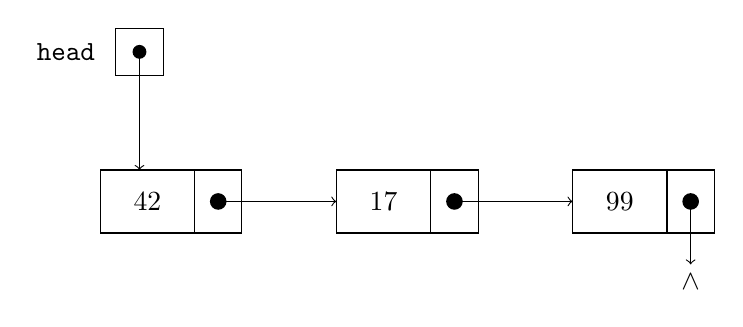
\begin{tikzpicture}                                                                                                                                                                                  
   

  %  head (quadratino sopra) ---                                                                                                                                                                    
  \draw (0.2, 2.0) rectangle (0.8, 2.6);
  \fill (0.5, 2.3) circle (2.5pt) coordinate (head);                                                                                                                                                   
  \node[left=4pt] at (0.2, 2.3) {\texttt{head}};
                                                                                                                                                                                                       
  % --- nodo 1 ---
  \draw (0,0) rectangle (1.8, 0.8);
  \draw (1.2, 0) -- (1.2, 0.8);
  \node at (0.6, 0.4) {42};
  \fill (1.5, 0.4) circle (3pt) coordinate (p1);                                                                                                                                                       
   
  % --- nodo 2 ---                                                                                                                                                                                     
  \draw (3,0) rectangle (4.8, 0.8);
  \draw (4.2, 0) -- (4.2, 0.8);
  \node at (3.6, 0.4) {17};                                                                                                                                                                            
  \fill (4.5, 0.4) circle (3pt) coordinate (p2);
                                                                                                                                                                                                       
  % --- nodo 3 ---                                                                                                                                                                                     
  \draw (6,0) rectangle (7.8, 0.8);
  \draw (7.2, 0) -- (7.2, 0.8);                                                                                                                                                                        
  \node at (6.6, 0.4) {99};
  \fill (7.5, 0.4) circle (3pt) coordinate (p3);
                                                                                                                                                                                                       
  % --- frecce ---
  \draw[->] (head) -- (0.5, 0.8);      % head → primo nodo                                                                                                                                             
  \draw[->] (p1)   -- (3.0, 0.4);      % nodo 1 → nodo 2
  \draw[->] (p2)   -- (6.0, 0.4);      % nodo 2 → nodo 3                                                                                                                                               
  \draw[->] (p3)   -- ++(0, -0.8)      % nodo 3 → nullptr                                                                                                                                              
    node[below] {$\wedge$};                                                                                                                                                                            
  \end{tikzpicture}  
\caption{Rappresentazione grafica di una lista concatenata: la cella \inlinecode{head} contiene il puntatore al primo nodo; ogni nodo è composto da un campo
  dato e un campo puntatore al nodo successivo; il simbolo $\wedge$ indica il valore \inlinecode{nullptr}, segnalando la fine della lista.}
  \label{fig:lista_semplice}
\end{center}
\end{figure}




\subsection{Implementazione}
Implemetiamo la lista come una classe \inlinecode{List}, che incapsula la struttura interna. Il nodo è definito come \inlinecode{struct cell}
privata, comoposta da un campo \inlinecode{int info} e un puntattore al nodo successivo \inlinecode{cell*next}. L'unico dato membro della classe è 
\inlinecode{cell*head}, il puntatore alla prima cella della lista.  

\begin{codebox}
    \begin{lstlisting}
class List{
    public:
    List();
    ~List();
    List(const List& other);
    void prepend(int value);
    void append(int value);
    void remove(int e);
    private:
    struct cell{
        int info;
        cell*next;
    };
    cell*head;
    cell*tail;
}
    \end{lstlisting}
\end{codebox}

\subsubsection{Costruttore}
Il costruttore inizializza \inlinecode{head} a \inlinecode{nullptr}, indicando che la lista nasce vuota. Non alloca nessuna cella: una lista con zero nodi è uno stato valido, e il puntatore nullo ne è la rappresentazione corretta.

\begin{codebox}
    \begin{lstlisting}
List::List() {
    head = nullptr;
    tail = nullptr;
}
    \end{lstlisting}
\end{codebox}

\subsubsection{Copy constructor}
l copy constructor viene invocato ogni volta che un oggetto viene inizializzato a partire da un altro dello stesso tipo: ad esempio nel passaggio per valore a una funzione, o in un'inizializzazione come \inlinecode{List b = a}.

Per una lista non basta copiare \inlinecode{head}: si otterebbe una \textbf{shallow copy}, in cui due
oggetti condividono le stesse celle in memoria. Quando il distruttore del primo libera quelle celle, il secondo si ritrova  con
puntatori dangling che puntano a memoria non più valida. Di consegeuenza occorre fare una \textbf{deep copy}, copiando non solo i puntatori,
ma anche le celle a cui puntano.


\begin{codebox}
    \begin{lstlisting}
List::List(const List& other) {
  head = nullptr;
  cell*cur = head;
  cell*cur_o = other.head;
  while(cur_o != nullptr){
    cell* nuova = new cell{cur_o->info, nullptr};
    if(cur == nullptr){
        head = nuova;
        cur = nuova;
    } else{
        cur->next = nuova;
        cur = cur->next;
    }
    cur_o = cur_o->next;
  }
}
    \end{lstlisting}
\end{codebox}

\subsubsection{Distruttore}
Il distruttore deve liberare tutta la memoria allocata dinamicamente. A differenza di un array, i nodi di una lista non sono contigui: ogni cella è stata allocata separatamente con \inlinecode{new}, quindi vanno deallocate una per una con \inlinecode{delete}. Se il distruttore non venisse definito, al termine della vita dell'oggetto il puntatore \inlinecode{head} verrebbe distrutto, ma le celle in memoria rimarrebbero irraggiungibili  producendo un \textbf{memory leak}.

\begin{codebox}
    \begin{lstlisting}
List::~List(){
    cell*cur = head;
    while(cur!=nullptr){
        cell*tmp = cur;
        cur= cur->next;
        delete tmp;
    }
}
    \end{lstlisting}
\end{codebox}
\subsubsection{Prepend}
\inlinecode{prepend} inserisce un nuovo nodo in testa alla lista. L'operazione alloca una nuova cella, la collega al nodo che era precedentemente in testa impostando il suo campo \inlinecode{next}, e aggiorna \inlinecode{head} in modo che punti alla nuova cella. Il costo è $O(1)$: non è necessario scorrere la lista.

\begin{figure}[h]
\begin{center}
  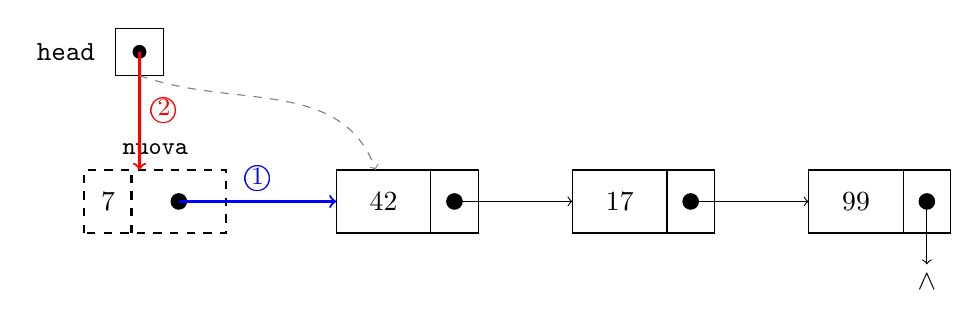
\begin{tikzpicture}

  % --- head ---
  \draw (-2.8, 2.0) rectangle (-2.2, 2.6);
  \fill (-2.5, 2.3) circle (2.5pt) coordinate (head);
  \node[left=4pt] at (-2.8, 2.3) {\texttt{head}};

  % --- nuova (nuovo nodo, bordo tratteggiato) ---
  \draw[dashed, thick] (-3.2, 0) rectangle (-1.4, 0.8);
  \draw[dashed, thick] (-2.6, 0) -- (-2.6, 0.8);
  \node at (-2.9, 0.4) {7};
  \fill (-2.0, 0.4) circle (3pt) coordinate (pnuova);
  \node[above=2pt] at (-2.3, 0.8) {\small\texttt{nuova}};

  % --- nodo 1 ---
  \draw (0,0) rectangle (1.8, 0.8);
  \draw (1.2, 0) -- (1.2, 0.8);
  \node at (0.6, 0.4) {42};
  \fill (1.5, 0.4) circle (3pt) coordinate (p1);

  % --- nodo 2 ---
  \draw (3,0) rectangle (4.8, 0.8);
  \draw (4.2, 0) -- (4.2, 0.8);
  \node at (3.6, 0.4) {17};
  \fill (4.5, 0.4) circle (3pt) coordinate (p2);

  % --- nodo 3 ---
  \draw (6,0) rectangle (7.8, 0.8);
  \draw (7.2, 0) -- (7.2, 0.8);
  \node at (6.6, 0.4) {99};
  \fill (7.5, 0.4) circle (3pt) coordinate (p3);

  % --- frecce catena esistente ---
  \draw[->] (p1) -- (3.0, 0.4);
  \draw[->] (p2) -- (6.0, 0.4);
  \draw[->] (p3) -- ++(0, -0.8) node[below] {$\wedge$};

  % --- (1) nuova->next = head ---
  \draw[->, thick, blue] (pnuova) -- (0, 0.4)
    node[midway, above] {\textcolor{blue}{\small\textcircled{1}}};

  % --- (2) head = nuova ---
  \draw[->, thick, red] (head) -- (-2.5, 0.8)
    node[midway, right] {\textcolor{red}{\small\textcircled{2}}};

  % --- vecchio valore di head (tratteggiato) ---
  \draw[->, dashed, gray] (-2.5, 2.0) to[out=-20, in=110] (0.5, 0.8);

  \end{tikzpicture}
\caption{\texttt{prepend(7)}: \textcircled{1}~\texttt{nuova->next = head} collega il nuovo nodo al vecchio primo nodo; \textcircled{2}~\texttt{head = nuova} aggiorna la testa. La freccia tratteggiata indica il vecchio valore di \texttt{head}.}
\label{fig:prepend}
\end{center}
\end{figure}

\begin{codebox}
    \begin{lstlisting}
void List::prepend(int value){
    cell * nuova = new cell{value, head};
    if(head == nullptr) tail = nuova;
    head = nuova;
}
    \end{lstlisting}
\end{codebox}
\subsubsection{Append}
\inlinecode{append} inserisce un nuovo nodo in coda alla lista. Senza un puntatore ausiliario è necessario scorrere tutta la lista per raggiungere l'ultimo nodo, quindi il costo è $O(n)$. Il caso lista vuota va gestito separatamente: se \inlinecode{head} è \inlinecode{nullptr} il nuovo nodo diventa direttamente la testa.

\begin{figure}[h]
\begin{center}
  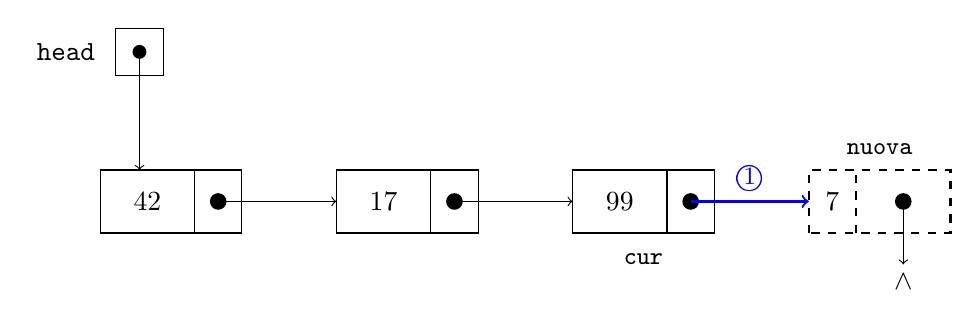
\begin{tikzpicture}

  % --- head ---
  \draw (0.2, 2.0) rectangle (0.8, 2.6);
  \fill (0.5, 2.3) circle (2.5pt) coordinate (head);
  \node[left=4pt] at (0.2, 2.3) {\texttt{head}};

  % --- nodo 42 ---
  \draw (0,0) rectangle (1.8, 0.8);
  \draw (1.2, 0) -- (1.2, 0.8);
  \node at (0.6, 0.4) {42};
  \fill (1.5, 0.4) circle (3pt) coordinate (p1);

  % --- nodo 17 ---
  \draw (3,0) rectangle (4.8, 0.8);
  \draw (4.2, 0) -- (4.2, 0.8);
  \node at (3.6, 0.4) {17};
  \fill (4.5, 0.4) circle (3pt) coordinate (p2);

  % --- nodo 99 (cur si ferma qui) ---
  \draw (6,0) rectangle (7.8, 0.8);
  \draw (7.2, 0) -- (7.2, 0.8);
  \node at (6.6, 0.4) {99};
  \fill (7.5, 0.4) circle (3pt) coordinate (p3);
  \node[below=4pt] at (6.9, 0) {\small\texttt{cur}};

  % --- nuova (bordo tratteggiato) ---
  \draw[dashed, thick] (9.0, 0) rectangle (10.8, 0.8);
  \draw[dashed, thick] (9.6, 0) -- (9.6, 0.8);
  \node at (9.3, 0.4) {7};
  \fill (10.2, 0.4) circle (3pt) coordinate (pnuova);
  \node[above=2pt] at (9.9, 0.8) {\small\texttt{nuova}};

  % --- frecce catena esistente ---
  \draw[->] (head) -- (0.5, 0.8);
  \draw[->] (p1) -- (3.0, 0.4);
  \draw[->] (p2) -- (6.0, 0.4);

  % --- (1) cur->next = nuova ---
  \draw[->, thick, blue] (p3) -- (9.0, 0.4)
    node[midway, above] {\textcolor{blue}{\small\textcircled{1}}};

  % --- nuova->next = nullptr ---
  \draw[->] (pnuova) -- ++(0, -0.8) node[below] {$\wedge$};

  \end{tikzpicture}
\caption{\texttt{append(7)}: \texttt{cur} avanza fino all'ultimo nodo (\texttt{cur->next == nullptr}); \textcircled{1}~\texttt{cur->next = nuova} collega il nuovo nodo in coda.}
\label{fig:append}
\end{center}
\end{figure}

\begin{codebox}
    \begin{lstlisting}
void List::append(int value){
    cell * cur=head;
    cell*nuova = new cell{value,nullptr};
    if(cur== head)
        head = nuova;
    else{
        while(cur->next !=nullptr){
            cur = cur->next;
        }
        cur->next = nuova;
    }
}
    \end{lstlisting}
    
\end{codebox}


\subsubsection{Remove}
\inlinecode{remove} elimina dalla lista il primo nodo il cui campo \inlinecode{info} è uguale al valore \inlinecode{e}. Per scollegare un nodo occorre aggiornare il campo \inlinecode{next} del suo predecessore; si mantiene quindi un puntatore \inlinecode{prev} che insegue \inlinecode{cur} di un passo. Tre casi particolari vanno gestiti esplicitamente: se il nodo cercato non esiste la funzione ritorna senza fare nulla; se il nodo da rimuovere è la testa, \inlinecode{head} viene aggiornato direttamente; se è la coda, il puntatore \inlinecode{tail} va retrocesso a \inlinecode{prev}. Il costo è $O(n)$ nel caso peggiore.

\begin{figure}[h]
\begin{center}
  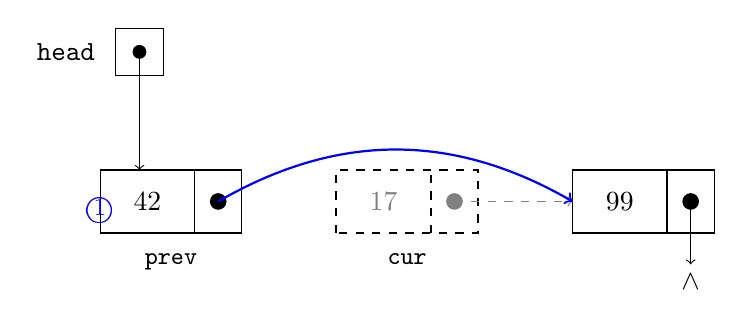
\begin{tikzpicture}

  % --- head ---
  \draw (0.2, 2.0) rectangle (0.8, 2.6);
  \fill (0.5, 2.3) circle (2.5pt) coordinate (head);
  \node[left=4pt] at (0.2, 2.3) {\texttt{head}};

  % --- nodo 42 (prev) ---
  \draw (0,0) rectangle (1.8, 0.8);
  \draw (1.2, 0) -- (1.2, 0.8);
  \node at (0.6, 0.4) {42};
  \fill (1.5, 0.4) circle (3pt) coordinate (p1);
  \node[below=4pt] at (0.9, 0) {\small\texttt{prev}};

  % --- nodo 17 (cur, da eliminare, bordo tratteggiato) ---
  \draw[dashed, thick] (3,0) rectangle (4.8, 0.8);
  \draw[dashed, thick] (4.2, 0) -- (4.2, 0.8);
  \node[gray] at (3.6, 0.4) {17};
  \fill[gray] (4.5, 0.4) circle (3pt) coordinate (p2);
  \node[below=4pt] at (3.9, 0) {\small\texttt{cur}};

  % --- nodo 99 ---
  \draw (6,0) rectangle (7.8, 0.8);
  \draw (7.2, 0) -- (7.2, 0.8);
  \node at (6.6, 0.4) {99};
  \fill (7.5, 0.4) circle (3pt) coordinate (p3);

  % --- frecce catena esistente ---
  \draw[->] (head) -- (0.5, 0.8);
  \draw[->, dashed, gray] (p2) -- (6.0, 0.4);
  \draw[->] (p3) -- ++(0, -0.8) node[below] {$\wedge$};

  % --- (1) prev->next = cur->next  (salta il nodo da eliminare) ---
  \draw[->, thick, blue] (p1) to[out=30, in=150] (6.0, 0.4)
    node[midway, above] {\textcolor{blue}{\small\textcircled{1}}};

  \end{tikzpicture}
\caption{\texttt{remove(17)}: \texttt{prev} punta al nodo 42, \texttt{cur} al nodo 17 da eliminare. \textcircled{1}~\texttt{prev->next = cur->next} salta il nodo grigio; segue \texttt{delete cur} per liberare la memoria.}
\label{fig:remove}
\end{center}
\end{figure}

\begin{codebox}
    \begin{lstlisting}
void List::remove(int e){
    cell* cur = head;
    cell* prev = nullptr;
    while(cur != nullptr && cur->info != e){
        prev = cur;
        cur = cur->next;
    }
    if(cur == nullptr) return;
    if(prev == nullptr) head = cur->next;
    else prev->next = cur->next;
    if(cur->next == nullptr) tail = prev;
    delete cur;
}
    \end{lstlisting}
\end{codebox}

Con queste tre operazioni  \inlinecode{prepend}, \inlinecode{append} e \inlinecode{remove}  la lista ha un'interfaccia completa per gestire sequenze dinamiche di elementi. La struttura a puntatori che la caratterizza rende naturale aggiungere e togliere nodi senza spostare dati in memoria, al prezzo di dover attraversare la catena ogni volta che si cerca un elemento.


\section{Overloading degli operatori}

\defn{Overloading}{
    L'overloading degli operatori è il meccanismo del C++ che consente di ridefinire il comportamento degli operatori come \inlinecode{+}, \inlinecode{=}, \inlinecode{==}, ecc.\ su tipi definiti dall'utente.
    Un operatore non è altro che una funzione con una sintassi speciale: scrivere \inlinecode{a + b} equivale a invocare \inlinecode{operator+(a, b)}.
}

Riprendendo la classe \inlinecode{List} definita nella sezione precedente, ne estendiamo l'interfaccia implementando il sovraccarico degli operatori \inlinecode{=}, \inlinecode{==}, \inlinecode{+}, \inlinecode{-} e \inlinecode{*}. Le dichiarazioni vanno aggiunte nella parte \inlinecode{public} della classe:

\begin{codebox}
    \begin{lstlisting}
List& operator=(const List& other);
bool  operator==(const List& other) const;
List  operator+(const List& other)  const;
List  operator-(const List& other)  const;
List  operator*(const List& other)  const;
    \end{lstlisting}
\end{codebox}

\subsection{Assegnamento (\texttt{=})}
L'operatore di assegnamento esegue una deep copy dell'oggetto sorgente, liberando prima la memoria dell'oggetto destinazione. Il controllo \inlinecode{this == \&other} gestisce il caso di autoassegnamento (\inlinecode{a = a}), che senza quella guardia libererebbe i dati prima di copiarli.

\begin{codebox}
    \begin{lstlisting}
List& List::operator=(const List& other){
    if(this == &other) return *this;
    cell* cur = head;
    while(cur != nullptr){
        cell* tmp = cur;
        cur = cur->next;
        delete tmp;
    }
    head = nullptr;
    tail = nullptr;
    cell* cur_o = other.head;
    while(cur_o != nullptr){
        append(cur_o->info);
        cur_o = cur_o->next;
    }
    return *this;
}
    \end{lstlisting}
\end{codebox}

\subsection{Uguaglianza (\texttt{==})}
Due liste sono uguali se hanno la stessa lunghezza e gli stessi elementi nello stesso ordine. Si scorrono in parallelo con due puntatori: se i valori divergono si ritorna \inlinecode{false}; al termine entrambi i puntatori devono essere \inlinecode{nullptr}.

\begin{codebox}
    \begin{lstlisting}
bool List::operator==(const List& other) const {
    cell* a = head;
    cell* b = other.head;
    while(a != nullptr && b != nullptr){
        if(a->info != b->info) return false;
        a = a->next;
        b = b->next;
    }
    return a == nullptr && b == nullptr;
}
    \end{lstlisting}
\end{codebox}

\subsection{Concatenazione (\texttt{+})}
L'operatore \inlinecode{+} restituisce una nuova lista formata dagli elementi di \inlinecode{*this} seguiti da quelli di \inlinecode{other}. Si copia \inlinecode{*this} sfruttando il copy constructor, poi si appendono tutti i nodi di \inlinecode{other}.

\begin{codebox}
    \begin{lstlisting}
List List::operator+(const List& other) const {
    List result = *this;
    cell* cur = other.head;
    while(cur != nullptr){
        result.append(cur->info);
        cur = cur->next;
    }
    return result;
}
    \end{lstlisting}
\end{codebox}

\subsection{Differenza (\texttt{-})}
L'operatore \inlinecode{-} restituisce una nuova lista con gli elementi di \inlinecode{*this} che non compaiono in \inlinecode{other}. Per ogni nodo della prima lista si scorre la seconda cercando una corrispondenza; se non la si trova, il valore viene aggiunto al risultato.

\begin{codebox}
    \begin{lstlisting}
List List::operator-(const List& other) const {
    List result;
    cell* cur = head;
    while(cur != nullptr){
        cell* o = other.head;
        bool found = false;
        while(o != nullptr && !found){
            if(o->info == cur->info) found = true;
            else o = o->next;
        }
        if(!found) result.append(cur->info);
        cur = cur->next;
    }
    return result;
}
    \end{lstlisting}
\end{codebox}

\subsection{Intersezione (\texttt{*})}
L'operatore \inlinecode{*} restituisce una nuova lista con i soli elementi presenti in entrambe le liste. Per ogni nodo di \inlinecode{*this} si cerca il valore in \inlinecode{other}; se trovato, viene aggiunto al risultato.

\begin{codebox}
    \begin{lstlisting}
List List::operator*(const List& other) const {
    List result;
    cell* cur = head;
    while(cur != nullptr){
        cell* o = other.head;
        bool found = false;
        while(o != nullptr && !found){
            if(o->info == cur->info) found = true;
            else o = o->next;
        }
        if(found) result.append(cur->info);
        cur = cur->next;
    }
    return result;
}
    \end{lstlisting}
\end{codebox}


\section{Liste doppiamente collegate}

\defn{Lista doppiamente collegata}{
    Una doubly-linked list è una lista in cui ogni nodo contiene, oltre al campo dato,
    due puntatori: \inlinecode{next} al nodo successivo e \inlinecode{prev} al nodo
    precedente. Il primo nodo ha \inlinecode{prev = nullptr}; l'ultimo ha
    \inlinecode{next = nullptr}.
}

Il vantaggio rispetto alla lista semplice è la possibilità di scorrere la lista in
entrambe le direzioni e di rimuovere un nodo in $O(1)$ dato il suo puntatore, senza
dover mantenere \inlinecode{prev} durante la scansione.

\begin{figure}[ht]
\begin{center}
  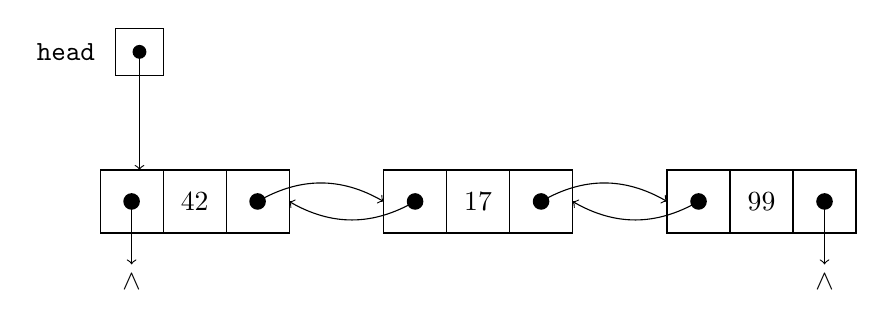
\begin{tikzpicture}

  % --- head ---
  \draw (0.2, 2.0) rectangle (0.8, 2.6);
  \fill (0.5, 2.3) circle (2.5pt) coordinate (head);
  \node[left=4pt] at (0.2, 2.3) {\texttt{head}};

  % --- nodo 1 ---
  \draw (0, 0) rectangle (2.4, 0.8);
  \draw (0.8, 0) -- (0.8, 0.8);
  \draw (1.6, 0) -- (1.6, 0.8);
  \fill (0.4, 0.4) circle (3pt) coordinate (bp1);
  \node at (1.2, 0.4) {42};
  \fill (2.0, 0.4) circle (3pt) coordinate (fp1);

  % --- nodo 2 ---
  \draw (3.6, 0) rectangle (6.0, 0.8);
  \draw (4.4, 0) -- (4.4, 0.8);
  \draw (5.2, 0) -- (5.2, 0.8);
  \fill (4.0, 0.4) circle (3pt) coordinate (bp2);
  \node at (4.8, 0.4) {17};
  \fill (5.6, 0.4) circle (3pt) coordinate (fp2);

  % --- nodo 3 ---
  \draw (7.2, 0) rectangle (9.6, 0.8);
  \draw (8.0, 0) -- (8.0, 0.8);
  \draw (8.8, 0) -- (8.8, 0.8);
  \fill (7.6, 0.4) circle (3pt) coordinate (bp3);
  \node at (8.4, 0.4) {99};
  \fill (9.2, 0.4) circle (3pt) coordinate (fp3);

  % --- head -> nodo 1 ---
  \draw[->] (head) -- (0.5, 0.8);

  % --- frecce next (avanti, sopra) ---
  \draw[->] (fp1) to[out=30,  in=150] (3.6, 0.4);
  \draw[->] (fp2) to[out=30,  in=150] (7.2, 0.4);
  \draw[->] (fp3) -- ++(0, -0.8) node[below] {$\wedge$};

  % --- frecce prev (indietro, sotto) ---
  \draw[->] (bp1) -- ++(0, -0.8) node[below] {$\wedge$};
  \draw[->] (bp2) to[out=210, in=330] (2.4, 0.4);
  \draw[->] (bp3) to[out=210, in=330] (6.0, 0.4);

  \end{tikzpicture}
\caption{Lista doppiamente collegata: ogni nodo ha un puntatore \texttt{prev}
(sinistra) e uno \texttt{next} (destra). Il primo nodo ha \texttt{prev = nullptr};
l'ultimo ha \texttt{next = nullptr}.}
\label{fig:dlist}
\end{center}
\end{figure}

\subsection{Implementazione}

Il nodo aggiunge il campo \inlinecode{prev} rispetto alla lista semplice.
La classe \inlinecode{DList} espone le stesse operazioni.

\begin{codebox}
    \begin{lstlisting}
class DList{
public:
    DList();
    ~DList();
    void prepend(int value);
    void append(int value);
    void remove(int e);
private:
    struct cell{
        int   info;
        cell* next;
        cell* prev;
    };
    cell* head;
    cell* tail;
};
    \end{lstlisting}
\end{codebox}

\subsubsection{Costruttore e distruttore}

\begin{codebox}
    \begin{lstlisting}
DList::DList() : head(nullptr), tail(nullptr) {}

DList::~DList(){
    cell* cur = head;
    while(cur != nullptr){
        cell* tmp = cur;
        cur = cur->next;
        delete tmp;
    }
}
    \end{lstlisting}
\end{codebox}

\subsubsection{Prepend}
\inlinecode{prepend} inserisce in testa in $O(1)$. Il nuovo nodo punta con
\inlinecode{next} al vecchio primo; se la lista non era vuota, il vecchio primo
aggiorna il suo \inlinecode{prev}.

\begin{figure}[ht]
\begin{center}
  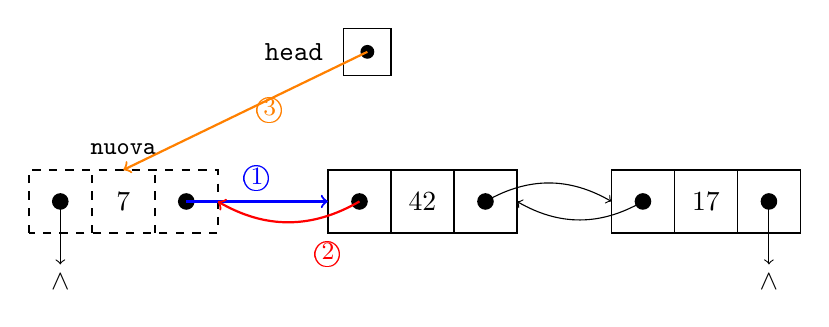
\begin{tikzpicture}

  % --- head ---
  \draw (0.2, 2.0) rectangle (0.8, 2.6);
  \fill (0.5, 2.3) circle (2.5pt) coordinate (head);
  \node[left=4pt] at (0.2, 2.3) {\texttt{head}};

  % --- nuova (tratteggiato) ---
  \draw[dashed, thick] (-3.8, 0) rectangle (-1.4, 0.8);
  \draw[dashed, thick] (-3.0, 0) -- (-3.0, 0.8);
  \draw[dashed, thick] (-2.2, 0) -- (-2.2, 0.8);
  \fill (-3.4, 0.4) circle (3pt) coordinate (bnuova);
  \node at (-2.6, 0.4) {7};
  \fill (-1.8, 0.4) circle (3pt) coordinate (fnuova);
  \node[above=2pt] at (-2.6, 0.8) {\small\texttt{nuova}};

  % --- nodo 42 ---
  \draw (0, 0) rectangle (2.4, 0.8);
  \draw (0.8, 0) -- (0.8, 0.8);
  \draw (1.6, 0) -- (1.6, 0.8);
  \fill (0.4, 0.4) circle (3pt) coordinate (bp1);
  \node at (1.2, 0.4) {42};
  \fill (2.0, 0.4) circle (3pt) coordinate (fp1);

  % --- nodo 17 ---
  \draw (3.6, 0) rectangle (6.0, 0.8);
  \draw (4.4, 0) -- (4.4, 0.8);
  \draw (5.2, 0) -- (5.2, 0.8);
  \fill (4.0, 0.4) circle (3pt) coordinate (bp2);
  \node at (4.8, 0.4) {17};
  \fill (5.6, 0.4) circle (3pt) coordinate (fp2);

  % --- frecce catena esistente ---
  \draw[->] (fp1) to[out=30,  in=150] (3.6, 0.4);
  \draw[->] (fp2) -- ++(0, -0.8) node[below] {$\wedge$};
  \draw[->] (bp2) to[out=210, in=330] (2.4, 0.4);

  % --- (1) nuova->next = head ---
  \draw[->, thick, blue] (fnuova) -- (0, 0.4)
    node[midway, above] {\textcolor{blue}{\small\textcircled{1}}};

  % --- (2) head->prev = nuova ---
  \draw[->, thick, red] (bp1) to[out=210, in=330] (-1.4, 0.4)
    node[midway, below] {\textcolor{red}{\small\textcircled{2}}};

  % --- (3) head = nuova ---
  \draw[->, thick, orange] (head) -- (-2.6, 0.8)
    node[midway, right] {\textcolor{orange}{\small\textcircled{3}}};

  % --- nuova->prev = nullptr ---
  \draw[->] (bnuova) -- ++(0, -0.8) node[below] {$\wedge$};

  \end{tikzpicture}
\caption{\texttt{prepend(7)}: \textcircled{1}~\texttt{nuova->next = head};
\textcircled{2}~\texttt{head->prev = nuova}; \textcircled{3}~\texttt{head = nuova}.}
\label{fig:dprepend}
\end{center}
\end{figure}

\begin{codebox}
    \begin{lstlisting}
void DList::prepend(int value){
    cell* nuova = new cell{value, head, nullptr};
    if(head != nullptr) head->prev = nuova;
    else tail = nuova;
    head = nuova;
}
    \end{lstlisting}
\end{codebox}

\subsubsection{Append}
\inlinecode{append} inserisce in coda in $O(1)$ grazie al puntatore \inlinecode{tail}.
Il nuovo nodo ha \inlinecode{next = nullptr} e \inlinecode{prev = tail}; il vecchio
ultimo aggiorna il suo \inlinecode{next}.

\begin{figure}[ht]
\begin{center}
  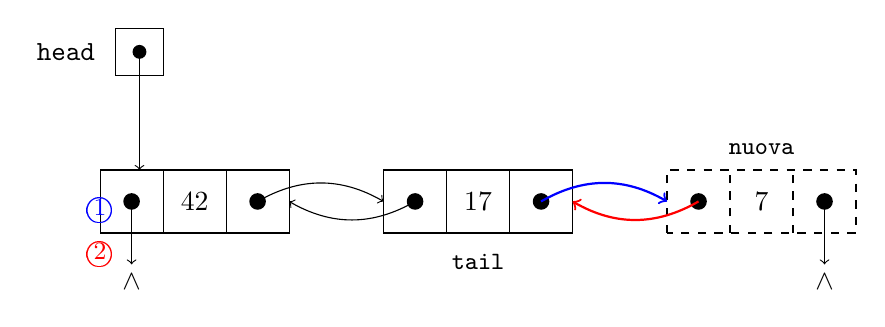
\begin{tikzpicture}

  % --- head ---
  \draw (0.2, 2.0) rectangle (0.8, 2.6);
  \fill (0.5, 2.3) circle (2.5pt) coordinate (head);
  \node[left=4pt] at (0.2, 2.3) {\texttt{head}};

  % --- nodo 42 ---
  \draw (0, 0) rectangle (2.4, 0.8);
  \draw (0.8, 0) -- (0.8, 0.8);
  \draw (1.6, 0) -- (1.6, 0.8);
  \fill (0.4, 0.4) circle (3pt) coordinate (bp1);
  \node at (1.2, 0.4) {42};
  \fill (2.0, 0.4) circle (3pt) coordinate (fp1);

  % --- nodo 17 (tail prima) ---
  \draw (3.6, 0) rectangle (6.0, 0.8);
  \draw (4.4, 0) -- (4.4, 0.8);
  \draw (5.2, 0) -- (5.2, 0.8);
  \fill (4.0, 0.4) circle (3pt) coordinate (bp2);
  \node at (4.8, 0.4) {17};
  \fill (5.6, 0.4) circle (3pt) coordinate (fp2);
  \node[below=4pt] at (4.8, 0) {\small\texttt{tail}};

  % --- nuova (tratteggiato) ---
  \draw[dashed, thick] (7.2, 0) rectangle (9.6, 0.8);
  \draw[dashed, thick] (8.0, 0) -- (8.0, 0.8);
  \draw[dashed, thick] (8.8, 0) -- (8.8, 0.8);
  \fill (7.6, 0.4) circle (3pt) coordinate (bp3);
  \node at (8.4, 0.4) {7};
  \fill (9.2, 0.4) circle (3pt) coordinate (fp3);
  \node[above=2pt] at (8.4, 0.8) {\small\texttt{nuova}};

  % --- frecce catena esistente ---
  \draw[->] (head) -- (0.5, 0.8);
  \draw[->] (fp1) to[out=30,  in=150] (3.6, 0.4);
  \draw[->] (bp1) -- ++(0, -0.8) node[below] {$\wedge$};
  \draw[->] (bp2) to[out=210, in=330] (2.4, 0.4);

  % --- (1) tail->next = nuova ---
  \draw[->, thick, blue] (fp2) to[out=30, in=150] (7.2, 0.4)
    node[midway, above] {\textcolor{blue}{\small\textcircled{1}}};

  % --- (2) nuova->prev = tail ---
  \draw[->, thick, red] (bp3) to[out=210, in=330] (6.0, 0.4)
    node[midway, below] {\textcolor{red}{\small\textcircled{2}}};

  % --- nuova->next = nullptr ---
  \draw[->] (fp3) -- ++(0, -0.8) node[below] {$\wedge$};

  \end{tikzpicture}
\caption{\texttt{append(7)}: \textcircled{1}~\texttt{tail->next = nuova};
\textcircled{2}~\texttt{nuova->prev = tail}; poi \texttt{tail = nuova}.}
\label{fig:dappend}
\end{center}
\end{figure}

\begin{codebox}
    \begin{lstlisting}
void DList::append(int value){
    cell* nuova = new cell{value, nullptr, tail};
    if(tail != nullptr) tail->next = nuova;
    else head = nuova;
    tail = nuova;
}
    \end{lstlisting}
\end{codebox}

\subsubsection{Remove}
Nella lista doppia, dato il nodo da eliminare, è sufficiente aggiornare i puntatori dei suoi vicini diretti. La ricerca rimane $O(n)$, ma il distacco del nodo è $O(1)$ senza scorrere da capo.

\begin{figure}[ht]
\begin{center}
  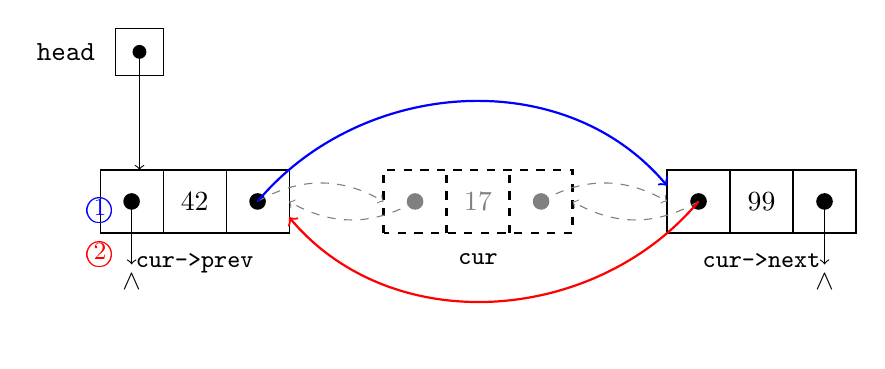
\begin{tikzpicture}

  % --- head ---
  \draw (0.2, 2.0) rectangle (0.8, 2.6);
  \fill (0.5, 2.3) circle (2.5pt) coordinate (head);
  \node[left=4pt] at (0.2, 2.3) {\texttt{head}};

  % --- nodo 42 (prev) ---
  \draw (0, 0) rectangle (2.4, 0.8);
  \draw (0.8, 0) -- (0.8, 0.8);
  \draw (1.6, 0) -- (1.6, 0.8);
  \fill (0.4, 0.4) circle (3pt) coordinate (bp1);
  \node at (1.2, 0.4) {42};
  \fill (2.0, 0.4) circle (3pt) coordinate (fp1);
  \node[below=4pt] at (1.2, 0) {\small\texttt{cur->prev}};

  % --- nodo 17 (cur, da eliminare) ---
  \draw[dashed, thick] (3.6, 0) rectangle (6.0, 0.8);
  \draw[dashed, thick] (4.4, 0) -- (4.4, 0.8);
  \draw[dashed, thick] (5.2, 0) -- (5.2, 0.8);
  \fill[gray] (4.0, 0.4) circle (3pt) coordinate (bp2);
  \node[gray] at (4.8, 0.4) {17};
  \fill[gray] (5.6, 0.4) circle (3pt) coordinate (fp2);
  \node[below=4pt] at (4.8, 0) {\small\texttt{cur}};

  % --- nodo 99 (next) ---
  \draw (7.2, 0) rectangle (9.6, 0.8);
  \draw (8.0, 0) -- (8.0, 0.8);
  \draw (8.8, 0) -- (8.8, 0.8);
  \fill (7.6, 0.4) circle (3pt) coordinate (bp3);
  \node at (8.4, 0.4) {99};
  \fill (9.2, 0.4) circle (3pt) coordinate (fp3);
  \node[below=4pt] at (8.4, 0) {\small\texttt{cur->next}};

  % --- frecce originali (grigie) ---
  \draw[->] (head) -- (0.5, 0.8);
  \draw[->, dashed, gray] (fp1) to[out=30,  in=150] (3.6, 0.4);
  \draw[->, dashed, gray] (fp2) to[out=30,  in=150] (7.2, 0.4);
  \draw[->, dashed, gray] (bp2) to[out=210, in=330] (2.4, 0.4);
  \draw[->, dashed, gray] (bp3) to[out=210, in=330] (6.0, 0.4);
  \draw[->] (bp1) -- ++(0, -0.8) node[below] {$\wedge$};
  \draw[->] (fp3) -- ++(0, -0.8) node[below] {$\wedge$};

  % --- (1) prev->next = cur->next ---
  \draw[->, thick, blue] (fp1) to[out=50, in=130] (7.2, 0.6)
    node[midway, above] {\textcolor{blue}{\small\textcircled{1}}};

  % --- (2) next->prev = cur->prev ---
  \draw[->, thick, red] (bp3) to[out=230, in=310] (2.4, 0.2)
    node[midway, below] {\textcolor{red}{\small\textcircled{2}}};

  \end{tikzpicture}
\caption{\texttt{remove(17)}: \textcircled{1}~\texttt{cur->prev->next = cur->next} salta il nodo grigio in avanti; \textcircled{2}~\texttt{cur->next->prev = cur->prev} chiude il collegamento all'indietro; segue \texttt{delete cur}.}
\label{fig:dremove}
\end{center}
\end{figure}

\begin{codebox}
    \begin{lstlisting}
void DList::remove(int e){
    cell* cur = head;
    while(cur != nullptr && cur->info != e)
        cur = cur->next;
    if(cur == nullptr) return;
    if(cur->prev != nullptr) cur->prev->next = cur->next;
    else head = cur->next;
    if(cur->next != nullptr) cur->next->prev = cur->prev;
    else tail = cur->prev;
    delete cur;
}
    \end{lstlisting}
\end{codebox}

\section{Liste circolari}

\defn{ lista circolare }{
Una lista circolare è un a lista concatenata in cui l'ultimo 
nodo non punta a \inlinecode{nullptr},bensì al primo nodo della lista,
formando  un anello chiuso senza inzio nè fine espliciti.
}
La differenza rispetto alla lista semplice è minima: cambia solo il valore del puntatore \inlinecode{next} dell'ultimo nodo, che invece di \inlinecode{nullptr} punta di nuovo a \inlinecode{head}.

\begin{figure}[ht]
\begin{center}
  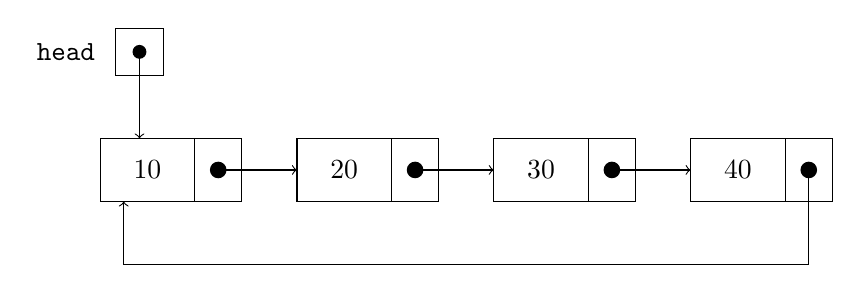
\begin{tikzpicture}

  % --- head (quadratino) ---
  \draw (0.2, 1.6) rectangle (0.8, 2.2);
  \fill (0.5, 1.9) circle (2.5pt) coordinate (head);
  \node[left=4pt] at (0.2, 1.9) {\texttt{head}};

  % --- nodo 10 ---
  \draw (0,0) rectangle (1.8, 0.8);
  \draw (1.2, 0) -- (1.2, 0.8);
  \node at (0.6, 0.4) {10};
  \fill (1.5, 0.4) circle (3pt) coordinate (p1);

  % --- nodo 20 ---
  \draw (2.5,0) rectangle (4.3, 0.8);
  \draw (3.7, 0) -- (3.7, 0.8);
  \node at (3.1, 0.4) {20};
  \fill (4.0, 0.4) circle (3pt) coordinate (p2);

  % --- nodo 30 ---
  \draw (5.0,0) rectangle (6.8, 0.8);
  \draw (6.2, 0) -- (6.2, 0.8);
  \node at (5.6, 0.4) {30};
  \fill (6.5, 0.4) circle (3pt) coordinate (p3);

  % --- nodo 40 ---
  \draw (7.5,0) rectangle (9.3, 0.8);
  \draw (8.7, 0) -- (8.7, 0.8);
  \node at (8.1, 0.4) {40};
  \fill (9.0, 0.4) circle (3pt) coordinate (p4);

  % --- head -> nodo 10 ---
  \draw[->] (head) -- (0.5, 0.8);

  % --- frecce consecutive ---
  \draw[->] (p1) -- (2.5, 0.4);
  \draw[->] (p2) -- (5.0, 0.4);
  \draw[->] (p3) -- (7.5, 0.4);

  % --- freccia di chiusura: 40 -> 10 (sotto) ---
  \draw[->] (9.0, 0.4) -- (9.0, -0.8) -- (0.3, -0.8) -- (0.3, 0);

  \end{tikzpicture}
\caption{Lista circolare: l'ultimo nodo (40) ha \texttt{next} che punta al primo nodo (10), chiudendo l'anello. Non esiste un \texttt{nullptr} a segnalare la fine.}
\label{fig:circular}
\end{center}
\end{figure}

\subsection{Implementazione}

La struttura interna è identica alla lista semplice: ogni nodo ha un campo \inlinecode{info} e un puntatore \inlinecode{next}. L'unica differenza è l'invariante mantenuta dalla classe: \inlinecode{tail->next == head} invece di \inlinecode{tail->next == nullptr}. Tenere \inlinecode{tail} come unico dato membro è la scelta più conveniente: da \inlinecode{tail} si raggiunge la testa in $O(1)$ tramite \inlinecode{tail->next}, evitando di scorrere tutta la lista per trovare il punto di inserimento in coda.

\begin{codebox}
    \begin{lstlisting}
class CList{
public:
    CList();
    ~CList();
    void insert_after(int ref, int value);
    void remove(int e);
private:
    struct cell{
        int   info;
        cell* next;
    };
    cell* tail;
};
    \end{lstlisting}
\end{codebox}

\subsubsection{Costruttore e distruttore}
Il costruttore inizializza \inlinecode{tail} a \inlinecode{nullptr}, che rappresenta la lista vuota. Il distruttore scorre l'anello partendo da \inlinecode{tail->next} (la testa) e si ferma quando ritorna a \inlinecode{tail}.

\begin{codebox}
    \begin{lstlisting}
CList::CList() : tail(nullptr) {}

CList::~CList(){
    if(tail == nullptr) return;
    cell* cur = tail->next;
    while(cur != tail){
        cell* tmp = cur;
        cur = cur->next;
        delete tmp;
    }
    delete tail;
}
    \end{lstlisting}
\end{codebox}

\subsubsection{Insert\_after}
\inlinecode{insert\_after(ref, value)} inserisce un nuovo nodo immediatamente dopo il primo nodo con valore \inlinecode{ref}. Si scorre l'anello finché non si trova il nodo di riferimento o si completa un giro; se trovato, il nuovo nodo viene incuneato aggiornando i due puntatori coinvolti. Se il nodo di riferimento è \inlinecode{tail}, il nuovo nodo diventa il nuovo \inlinecode{tail}. Il costo è $O(n)$ per la ricerca.

\begin{figure}[ht]
\begin{center}
  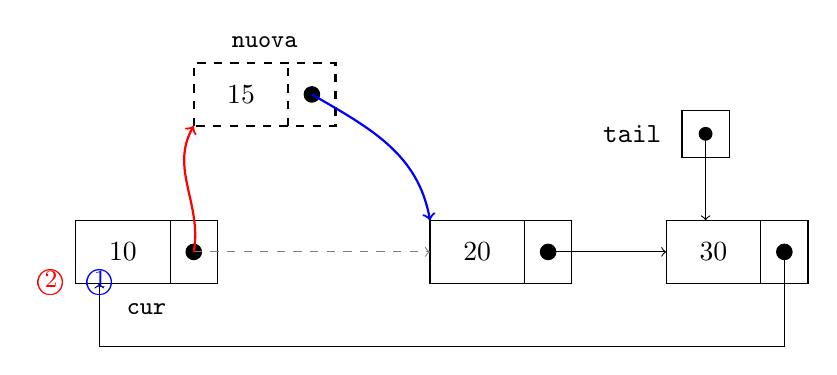
\begin{tikzpicture}

  % --- tail box (sopra nodo 30) ---
  \draw (7.7, 1.6) rectangle (8.3, 2.2);
  \fill (8.0, 1.9) circle (2.5pt) coordinate (itail);
  \node[left=4pt] at (7.7, 1.9) {\texttt{tail}};
  \draw[->] (itail) -- (8.0, 0.8);

  % --- nuova (15), bordo tratteggiato, sopra ---
  \draw[dashed, thick] (1.5, 2.0) rectangle (3.3, 2.8);
  \draw[dashed, thick] (2.7, 2.0) -- (2.7, 2.8);
  \node at (2.1, 2.4) {15};
  \fill (3.0, 2.4) circle (3pt) coordinate (ip15);
  \node[above=2pt] at (2.4, 2.8) {\small\texttt{nuova}};

  % --- nodo 10 (cur) ---
  \draw (0,0) rectangle (1.8,0.8);
  \draw (1.2,0) -- (1.2,0.8);
  \node at (0.6,0.4) {10};
  \fill (1.5,0.4) circle (3pt) coordinate (ip10);
  \node[below=4pt] at (0.9,0) {\small\texttt{cur}};

  % --- nodo 20 ---
  \draw (4.5,0) rectangle (6.3,0.8);
  \draw (5.7,0) -- (5.7,0.8);
  \node at (5.1,0.4) {20};
  \fill (6.0,0.4) circle (3pt) coordinate (ip20);

  % --- nodo 30 (tail) ---
  \draw (7.5,0) rectangle (9.3,0.8);
  \draw (8.7,0) -- (8.7,0.8);
  \node at (8.1,0.4) {30};
  \fill (9.0,0.4) circle (3pt) coordinate (ip30);

  % --- frecce invariate ---
  \draw[->] (ip20) -- (7.5,0.4);
  \draw[->] (9.0,0.4) -- (9.0,-0.8) -- (0.3,-0.8) -- (0.3,0);

  % --- vecchia 10->20 (grigia, viene sostituita) ---
  \draw[->, dashed, gray] (ip10) -- (4.5,0.4);

  % --- ① nuova->next = cur->next (15->20) ---
  \draw[->, thick, blue] (ip15) to[out=330, in=100] (4.5,0.8)
    node[midway, right] {\textcolor{blue}{\small\textcircled{1}}};

  % --- ② cur->next = nuova (10->15) ---
  \draw[->, thick, red] (ip10) to[out=80, in=240] (1.5,2.0)
    node[midway, left] {\textcolor{red}{\small\textcircled{2}}};

  \end{tikzpicture}
\caption{\texttt{insert\_after(10,\,15)}: \texttt{cur} punta al nodo 10. \textcircled{1}~\texttt{nuova->next = cur->next} collega il nuovo nodo al successore; \textcircled{2}~\texttt{cur->next = nuova} incunea il nodo nell'anello. La freccia grigia indica il collegamento sostituito.}
\label{fig:cinsert}
\end{center}
\end{figure}

\begin{codebox}
    \begin{lstlisting}
void CList::insert_after(int ref, int value){
    if(tail == nullptr) return;
    cell* cur = tail->next;
    bool done = false;
    while(!done && cur->info != ref){
        if(cur == tail) done = true;
        else cur = cur->next;
    }
    if(cur->info != ref) return;
    cell* nuova = new cell{value, cur->next};
    cur->next = nuova;
    if(cur == tail) tail = nuova;
}
    \end{lstlisting}
\end{codebox}

\subsubsection{Remove}
La visita dell'anello si ferma quando si è fatto un giro completo. Occorre distinguere tre casi: lista con un solo nodo, rimozione della testa e rimozione di un nodo interno o della coda.

\begin{figure}[ht]
\begin{center}
  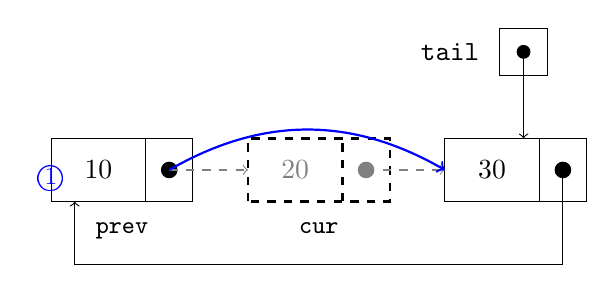
\begin{tikzpicture}

  % --- tail box (sopra nodo 30) ---
  \draw (5.7, 1.6) rectangle (6.3, 2.2);
  \fill (6.0, 1.9) circle (2.5pt) coordinate (rtail);
  \node[left=4pt] at (5.7, 1.9) {\texttt{tail}};
  \draw[->] (rtail) -- (6.0, 0.8);

  % --- nodo 10 (prev) ---
  \draw (0,0) rectangle (1.8,0.8);
  \draw (1.2,0) -- (1.2,0.8);
  \node at (0.6,0.4) {10};
  \fill (1.5,0.4) circle (3pt) coordinate (rp10);
  \node[below=4pt] at (0.9,0) {\small\texttt{prev}};

  % --- nodo 20 (cur, da eliminare) ---
  \draw[dashed, thick] (2.5,0) rectangle (4.3,0.8);
  \draw[dashed, thick] (3.7,0) -- (3.7,0.8);
  \node[gray] at (3.1,0.4) {20};
  \fill[gray] (4.0,0.4) circle (3pt) coordinate (rp20);
  \node[below=4pt] at (3.4,0) {\small\texttt{cur}};

  % --- nodo 30 ---
  \draw (5.0,0) rectangle (6.8,0.8);
  \draw (6.2,0) -- (6.2,0.8);
  \node at (5.6,0.4) {30};
  \fill (6.5,0.4) circle (3pt) coordinate (rp30);

  % --- vecchia 10->20 (grigia) ---
  \draw[->, dashed, gray] (rp10) -- (2.5,0.4);

  % --- vecchia 20->30 (grigia) ---
  \draw[->, dashed, gray] (rp20) -- (5.0,0.4);

  % --- ① prev->next = cur->next (10->30) ---
  \draw[->, thick, blue] (rp10) to[out=30, in=150] (5.0,0.4)
    node[midway, above] {\textcolor{blue}{\small\textcircled{1}}};

  % --- chiusura 30->10 (sotto, invariata) ---
  \draw[->] (6.5,0.4) -- (6.5,-0.8) -- (0.3,-0.8) -- (0.3,0);

  \end{tikzpicture}
\caption{\texttt{remove(20)}: \texttt{prev} punta a 10, \texttt{cur} al nodo 20 da eliminare. \textcircled{1}~\texttt{prev->next = cur->next} salta il nodo grigio; la chiusura dell'anello rimane invariata. Segue \texttt{delete cur}.}
\label{fig:cremove}
\end{center}
\end{figure}

\begin{codebox}
    \begin{lstlisting}
void CList::remove(int e){
    if(tail == nullptr) return;
    cell* cur  = tail->next;
    cell* prev = tail;
    bool  done = false;
    while(!done && cur->info != e){
        if(cur == tail) done = true;
        else {
            prev = cur;
            cur  = cur->next;
        }
    }
    if(cur->info != e) return;
    if(cur == tail && cur == tail->next){
        tail = nullptr;
    } else {
        prev->next = cur->next;
        if(cur == tail) tail = prev;
    }
    delete cur;
}
    \end{lstlisting}
\end{codebox}